\subsection{Leaderboards}
\label{real_leader}
\paragraph{} En fin de partie l'utilisateur a la possibilit� d'enregistrer son score sur une plateforme web et de consulter le classement des meilleurs score � Urban Life Simulator.

\subsubsection{Le Site Web}
\label{sec:siteweb}
\paragraph{}Les classements aux diff�rents niveaux de difficult�s sont disponibles sur un site web heberg� et accessible 24/24h.
\begin{figure}[H]
	\centering
		
\includegraphics[width=0.75\textwidth]{images/realheader.png}
		\caption{Les diff�rentes pages accessibles du site web}
	\label{fig:realheader}
\end{figure}
\paragraph{}Le site est compos� de 5 pages:
\begin{itemize}
\item La page d'accueil
\item Le classement du mode Easy
\item Le classement du mode Normal
\item Le classement du mode Hard
\item Le classement du mode Pro
\end{itemize}
\paragraph{}La page d'enregistrement des scores est accessible seulement par un lien g�n�r� par le jeu en fin de partie, l'utilisateur pourra ensuite scanner un QR Code pour acc�der � la page ou cliquer sur un bouton qui le renverra sur la page si il ne poss�de pas de lecteur de code QR.

\subsubsection{Principe du classement}
\label{sec:leaderprincipe}
\paragraph{}Le principe du classement est de classer les meilleurs joueurs � Urban Life Simulator, voici les r�gles du classement de Urban Life Simulator:
\begin{itemize}
\item Les plus hauts scores se retrouveront en haut de la liste.
\item Le classement ne retient que les 10 meilleurs scores.
\item Les scores en dessous du dizi�me meilleur score ne sont pas retenus ou sont effac�s lorsque le 10eme score est battu.
\item En cas d'�galit� de score dans le classement, le joueur ayant fait le score en premier occupe la place sup�rieure. Ainsi en cas d'�galisation d'un score, le joueur performant l'�galisation se verra attribu� la place inf�rieure � tous les autres joueurs ayant d�j� fait le m�me score auparavant.
\end{itemize}

\subsubsection{Mod�lisation d'un classement}
\label{sec:realmodelscore}
\begin{figure}[H]
	\centering
		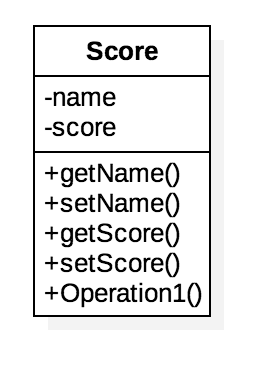
\includegraphics[width=0.30\textwidth]{images/score_class.png}
		\caption{Diagramme UML de la Classe Score en PHP}
	\label{fig:realscore}
\end{figure}
\paragraph{}Un score est mod�lis� par une classe "Score" en PHP ayant pour attribut:
\begin{itemize}
\item Un nom
\item Un score
\end{itemize}
\paragraph{}La classe "Score" poss�de pour seules m�thodes, les accesseurs et mutateurs des deux attributs pr�c�dants. Les 10 meilleurs scores sont ensuite ajout�s dans un tableau. Le tableau est ensuite s�rializ� dans un fichier sur le serveur.

\subsubsection{Ajout d'un score dans un classement}
\label{sec:realaddscore}
\paragraph{}L'ajout d'un score dans un classement est classique et se fait via un parcours du tableau contenant tous les scores par la fin, le parcours s'arr�te quand le score du joueur est inf�rieur au prochain score. Lors du parcours tous les scores sont d�cal�s vers le bas jusqu'� l'arr�t du parcours du tableau. Une fois que le parcours du tableau est arr�t�, le score de l'utilisateur est ins�r� � la place correspondante. 